\section{Graph Types}
Graph types are various and complex. Different type of graphs have their particular characteristics, which requires to be handled by special techniques. With the rapid development of graph mining, more and more complex graphs are constructed from real scenarios and analyzed by researchers, which offers the possibility to summarize several main types and relevant works in this section. Particularly, the following paragraphs introduce five main types of graph which are most frequently appeared in research studies and tightly connected with real-world scenarios, including heterogeneous \& multi-layer graph, sparse graph, dynamic graph, large graph and attribute graph. 

\subsection{Heterogeneous \& Multi-layer Graph} 

The research works about heterogeneous and multi-layer graph community detection are summarized together. The reason is that both types of graphs share very similar structure but still keep their own characteristics. For a heterogeneous graph, it should contains more than one type of node or edges. While for a multi-layer graph, it is composed from multiple single layer graphs. A single layer graph is with only one type of node/edge.  By connecting nodes across single layer graphs with edges, it formulates a multi-layer graph in the end. Figure \ref{fig:c2_hetero} clearly shows the definition difference between heterogeneous graph and multi-layer graph. In fact, multi-layer graph can be regarded as a particular type of heterogeneous graph. 

\begin{figure}
	% \setlength{\belowcaptionskip}{-10pt}
	\center
	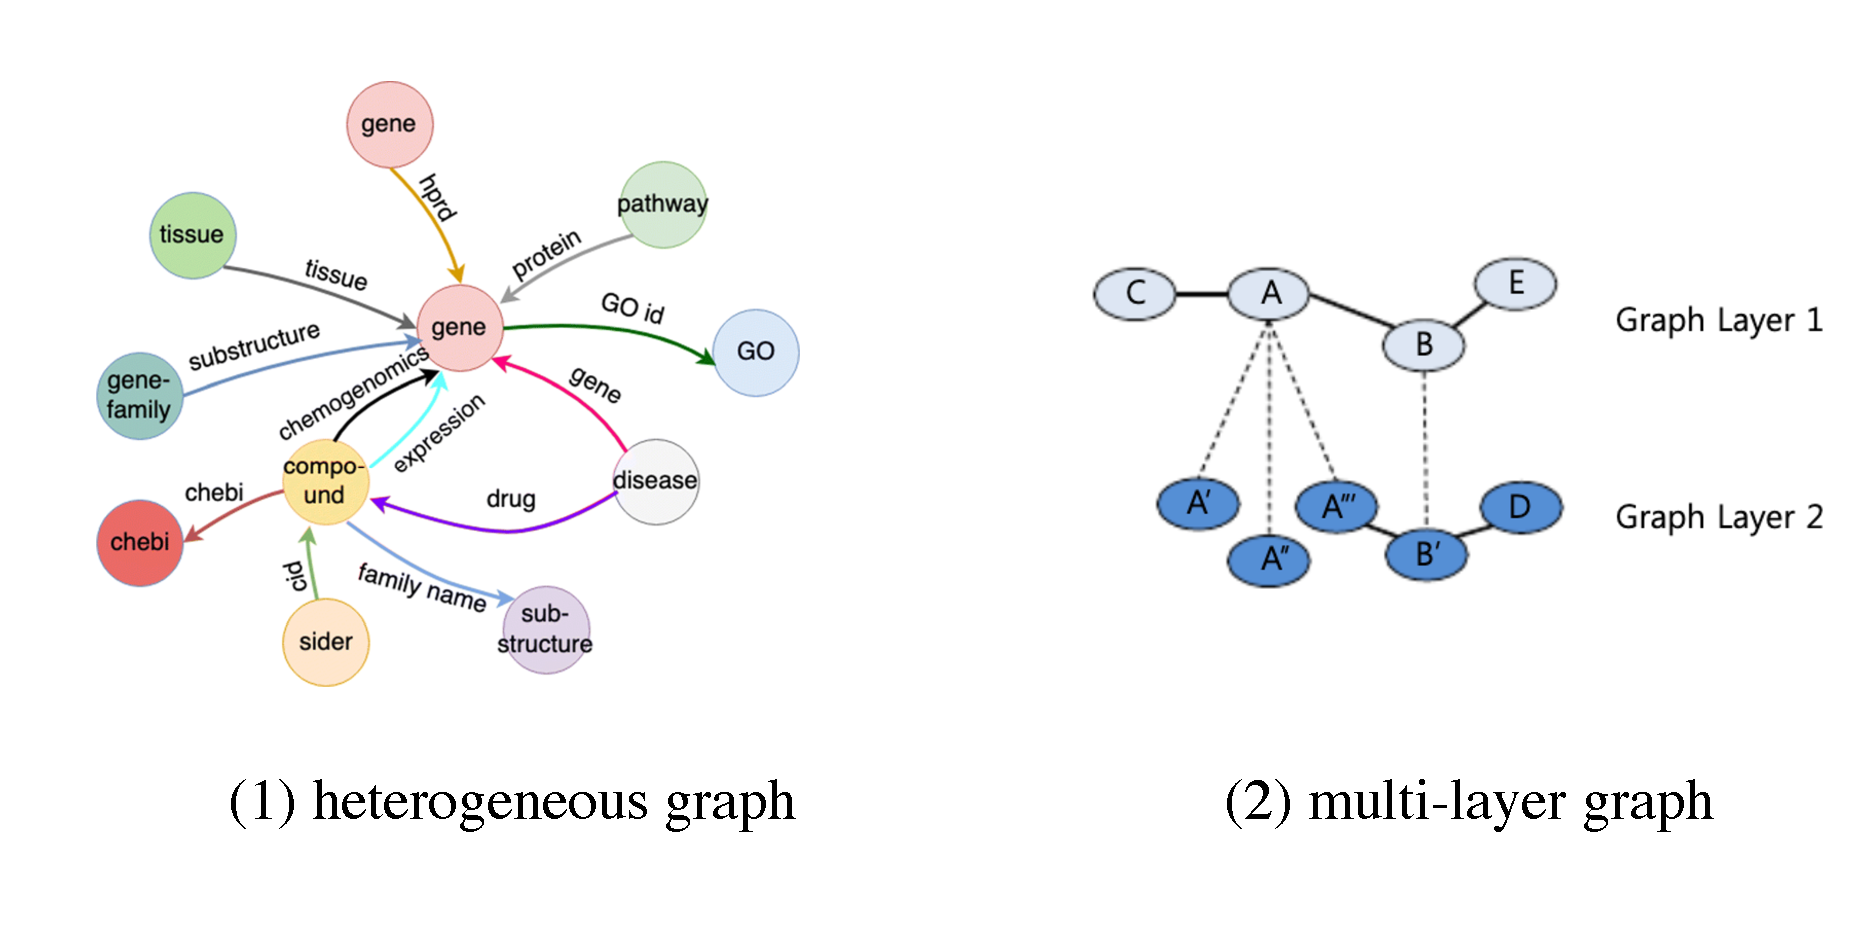
\includegraphics[width=\columnwidth]{img/chapter2/heterogenous.pdf} 
	\caption{Figure in the left is a typical heterogeneous medical graph in which nodes and edges refer to medical entities and their binding relationships from \cite{gao2019edge2vec}. Figure in the right is a multi-layer graph with two graph layers from \cite{kim2015community}.}
	\label{fig:c2_hetero}
\end{figure}  


Heterogeneous graph, also called heterogeneous information network, is a particularly complex graph which is ubiquitously appeared in current research works. By definition, a heterogeneous graph $G(V,E)$ has an extra node mapping function $\phi : V \rightarrow \mathcal{A}$ and an edge mapping function $\psi : E \rightarrow \mathcal{R} $ where each node $v \in V$ belongs to a particular node type $\phi(v) \in \mathcal{A}$ and each edge $e \in E$ belongs to a particular edge type $\psi(e) \in \mathcal{R}$. $\mathcal{A}$ is the collection of all node types and $\mathcal{R}$ is the collection of all edge types. A heterogeneous graph contains multiple node/edge types, which means at least either $|\mathcal{A}| > 1$ or $|\mathcal{R}| > 1$.

\cite{sun2013pathselclus} defines a graph structure called metapath, which is a path that connects node types with different types of edges and can be regarded as a general structure to represent path semantics. For example, a metapath in a scholarly graph can be ``Organization-(affiliated with)$\rightarrow$Author-(publish at)$\rightarrow$Venue'' where it contains three node types (``Organization'', ``Author'' and ``Venue'') and two types of edges (``affiliated with'' and ``publish at''). Particularly in this study, it integrates metapath selection with user guided clustering (a small set of nodes whose communities are known as prior information). In the end, it aims to learn the weights on selected metapaths to best satisfy the prior community knowledge via an EM approach.  

\cite{gupta2013community} introduces a joint approach to learn node affiliation distributions on popular communities in heterogeneous graph and detect node outliers which do not belong to any of the popular community distribution patterns in a holistic manner. It decomposes the heterogeneous graph into several homogeneous ones. The community detection step is derived from nonnegative matrix factorization framework and the refined outlier detection is learned via an iterative two-stage approach. In the NMF based community detection process, all prior-known community membership matrices of single node-type graphs $\{T_1,....,T_k\}$ can be used to calculate node community distribution under each node type:

\begin{equation}
	\argmin_{W,H}\sum_{i=1}^{k}||T_i - W_{i}H_{i}||^2 + \alpha \sum_{i \leq j \leq k}^{k}||H_i - H_j||^2
\end{equation}
which should subject to $W_i \geq 0$ and $H_i \geq 0$ for $ \forall i \leq k$. $W_i$ is the node vector representation matrix in the $i_{th}$ node-type graph and $H_i$ is the related community centroid matrix. The later part is the regularized term.

A node outlier score is calculated as the distance ($Dist(\cdot)$) between the current node community membership and its nearest community centroid:

\begin{equation}
S(i) =  \argmin_{j} Dist(T_{k_{(i,\cdot)}}, H_{k_{(j,\cdot)}})
\end{equation} 
Top $\rho$ nodes with largest outlier score will be regarded as outliers in current step. In an iterative learning process, the NMF method is optimized by reducing the detected outliers from the whole graph to support new node outlier detection. It stops when no outlier nodes are found out.

\cite{sun2012relation} solves a heterogeneous and incomplete graph community detection problem where only partial attribute information are given. The output of this paper includes two parts: node soft clustering distribution to indicate the probability of node affiliations to communities, and weights of edge types appeared in the graph. In model optimization, all edge types are assigned same weights in the beginning. The clustering process thereafter is applied to update the edge type weights according to the calculated average edge type consistency, which in return  guides the clustering process. The iterative process reaches to the end once all updated parameters are stable. 

Instead of node community detection, \cite{he2015stochastic} proposes an EM model for edge community detection. It aims to re-generate the whole graph by finding a partition to maximize the edge generation probabilities. Given an edge $e_{ij}$ with start node $i$ and end node $j$, its expected generation score in community $z$ is calculated as $A_{ij}^{z} = w_z\theta_{iz}\theta_{jz}$. $w_z$ is the size of community $z$ and $\theta_{iz}$ is the probability that community $z$ contains the node $i$. Then the probability of a link $e_{ij}$ belongs to community $z$ is calculated by dividing the whole generation score in all communities, as:
\begin{equation}
	R_{ij}^z = \frac{A_{ij}^{z} }{\sum_{k}{A_{ij}^{k} }}
\end{equation}
The edge $e_{ij}$ will be assigned to the community with largest generation probability. And all parameters can be learned through an EM approach.

\cite{zhou2013social} presents a social influence based framework to detect user communities in social graphs. In this paper, a social graph represents user collaborations (authors are connected by collaboration relationships) and an activity graph represents associated activity similarities (venues are connected by their topic similarities). The edges between social graph nodes and activity graph nodes represents their influence flow, such as publishing histories of authors towards venues. The three parts (social graph, activity graph and edges between them) constructs the final influence graph. First, it introduces  a new metric to  measure node similarity jointly using self-influence (social graph) and co-influence (influence graph) information. Later on, a designed SI-Cluster model takes advantage of the metric to learn node communities in the social graphs only via an Kmeans-like process. 

OCD-HSN model \cite{huang2018overlapping} detect node communities in four main steps. First, a set of seed nodes are selected according to their local minimum conductance, which enables a parallel community computation. Second, overlapping community detection is applied using local node expansion (adding and removing nodes iteratively). Third, node degrees are recalculated and normalized. Fourth, current communities are regarded as a node with coarser resolution to construct the next-level graph. Followed by all the previous steps, a hierarchical community partition can be formed in the end. 

 \cite{li2017semi} proposes a semi-supervised model to detect attribute heterogeneous graph communities by considering three types of information: node attributes, graph topological structure, and prior knowledge of must-links and cannot-links. It first calculates and assigns weights to node pairwise attribute similarity matrix and connected similarity matrix (calculated from meta-paths) to construct a node similarity matrix $S$. Then it considers the constraints (must-links and cannot-links) by assigning penalties to related node pairs. In the end, the unified model is optimized through an Expectation-Maximization (EM) framework to learn all the model parameters. 

Muilti-layer graph $G=\{G^1,G^2,...,G^k\}$ is composed by $k$ single-layer graphs $G^k= (V^k,E^k)$. For each possible pairwise single-layer graphs $G^i$ and $G^j$, there is a mapping function $\phi : G^i \rightarrow G^j$, meaning the nodes in graph $G^i$ can link to nodes in graph $G^j$, which formulates the connections between single-layer graphs. An extreme case of a multi-layer graph is that each single layer graph contains the same nodes.

\cite{kim2015community} is a short survey paper to introduce the definition of mullti-layer graph and differentiate its concept from heterogeneous graph. It offers a bunch of multi-layer graph datasets and points out several main tracks of methods, including pattern mining and matrix factorization. Typically, it introduces a popular two-layer graph community detection problem and introduces six main track methods, including cluster expansion, matrix factorization, unified distance, model-based methods, pattern mining and graph merging. 

\cite{bazzi2016community} constructs multi-layer graphs by tracking node dynamic changes across time. Therefore, each single layer graph shares the same nodes whose status and connections are changed over time. To solve the community detection in dynamic graphs, it generalizes the original Modularity method to adapt multi-layer graphs.  It also defines a persistence metric which measures the graph changes and stability across time.  

Multiplex Infomap \cite{de2015identifying} is derived from existing Infomap algorithm which originally designed for single-layer graphs. It uses codebooks to index each node and community in each layer, so that to record the paths of a random walker wandering in the multi-layer graph. The best community structure should obtains the shortest description length for the random paths. Similarly, \cite{valles2016multilayer} is also a generalized model from existing methods which is originally designed for single-layer graph community detection. Within the paper, it considers the simplest two-layer graph. It defines two type of models including an AND graph which only contains edges appeared in both layers, and a OR graph which contains edges appeared in either layers. In the end, it learns the two community partition result $C_1$ and $C_2$ in individual layers to maximize the probability to generate the AND graph from the two partitions and OR graph. 

\cite{huang2018harmonic} develops a multi-layer Modularity model by utilizing a defined graph structure called Harmonic Motif. By definition, a harmonic motif is a dense graph with largest average Z-score values in all $k$ graph layers. The Z-score shows the statistical significance of a subgraph towards the whole graph, which is calculated as:
\begin{equation}
Z = \frac{N_{real}- mean(N_{rand})}{std(N_{rand})}
\end{equation}
where $N_{real}$ is the number of time that the subgraph appears in each layer. $mean(N_{rand})$ and $std(N_{rand})$ refers to the mean and standard derivation of the number of times that the subgraph appears in a random graph with same node and number of edges.

From $k$ graph layers, the paper extracts all harmonic motifs to form a new graph layer. The existing $k$ layers are in the end coupled with the new layer to detect communities in the new graph layer by maximizing the integrated Modularity. 

\subsection{Sparse Graph}
Sparse graph is a very common phenomenon in graph mining, which is in contrary to dense graphs. However, their is no clear distinction between dense graph and sparse graph. A common notion is that dense graph is with the number of edges as $|E| = \mathcal{O}(|V|^2)$ as the maximum number of edges in a directed graph is $|V|(|V|-1)/2$. And a sparse graph usually contains the number of edges as $|E| = \mathcal{O}(|V|)$. Due to the fact that most of constructed graphs in real-world scenarios are sparse and incomplete, understanding sparse graph community detection gains a lot of practical value. 

Due to the fact that spectral clustering methods are not able to perform well in sparse graphs, \cite{krzakala2013spectral} argues that spectral methods on a refined matrix based on non-backtracking walks may achieve much better results than on the original adjacency matrix or Laplacian matrix.  The non-backtracking matrix $B$ is a $2|E| \times 2|E|$ matrix, defined as follows:
\begin{equation}
B_{(u\rightarrow v),(w\rightarrow x)} = 
\begin{cases}
1& \text{if v = w and u  $\neq$ x}\\
0& \text{otherwise}
\end{cases}
\end{equation}

\cite{chen2012clustering} designs a model for undirected, unweighted sparse graph community detection. It points out two types of clustering errors: \textit{(a)} an edge between nodes in different communities and \textit{(b)} a missing edge between nodes in the same community. These errors can be represented as an error matrix $S$ with corresponding values $\{+1,-1,0\}$. To treat the two types of errors differently, a cost matrix $M$ is utilized as well by assigning different weights on different error types. The object function thereafter is as follows to minimize the two types of errors:
\begin{equation}
	\argmin_{C,S} ||C|| + ||M \cdot S||
\end{equation}
with the restraints that $0 \leq C_{ij} \leq 1$. $C$ is the cluster matrix where $C_{ij} = 1$ if $v_i$ and $v_j$ are in the same community, and 0 otherwise. 

\cite{amini2013pseudo} claims involving perturbations in spectral clustering can improve its model performance in sparse graphs. The proposed model adds pseudo week edges between nodes to connect all disjoint components which suppose to be in the same community.  Particularly, it adds $0.25*(\lambda /|V|)$ where $\lambda$ is the average node degree in the sparse graph to each datapoint of the adjacency matrix $A$.

\cite{mirshahvalad2012significant} combines a perturbation strategy and link prediction in sparse graphs to assess all communities and select the most significant ones. As triangle is the smallest structural unit in a graph, the paper decides to complete partial of the open triangles in the original graph to achieve a denser graph. An open triangle completion means if there are two edges $e_{ij}$ and $e_{ik}$ links between a selected node triplet $<v_i,v_j,v_k>$, it will add an edge $e_{jk}$ to the original graph. By using this enhancing method, better community partition can be achieved from the denser graph. 

A rich number of researchers tend to explore sparse graph community detection from mathematical perspective. \cite{banks2016information} theoretically proves the lower and upper bound of information-theoretic threshold for community detection in the stochastic block model. The threshold is defined as $(\frac{2log(q-1)}{\lambda^2(q-1)}, \frac{2(1+\mathcal{O}(1/logq))}{\lambda})$.  $q$ is the community number, and $\lambda = \mathcal{O}(1/q)$. There will be no optimal communities for graph structure if the average node degree falls out of the threshold boundary. \cite{chin2015stochastic} is another theory paper which offers two spectral algorithms to solve sparse graph community detection model. Derived from Grothendieck’s inequality, \cite{guedon2016community} proves random graph semidefinite optimization consistency and illustrates its proofs in sparse graph community detection. 

\subsection{Dynamic Graph}

Dynamic graph, also named as temporal graph in this paper, refers to a particular type of graphs which can be dynamically changed. This graph characteristic will lead to node community evolution, which is usually happened in social media or other real-world scenarios where the user profiles and interactions are updated frequently. \cite{hartmann2016clustering} summarizes a set of relevant papers  about the metrics, tasks and datasets. It especially lists a number of papers focusing online clustering. Figure \ref{fig:c2_dynamic} illustrates a typical framework of dynamic community detection.
 
 \begin{figure}
 	% \setlength{\belowcaptionskip}{-10pt}
 	\center
 	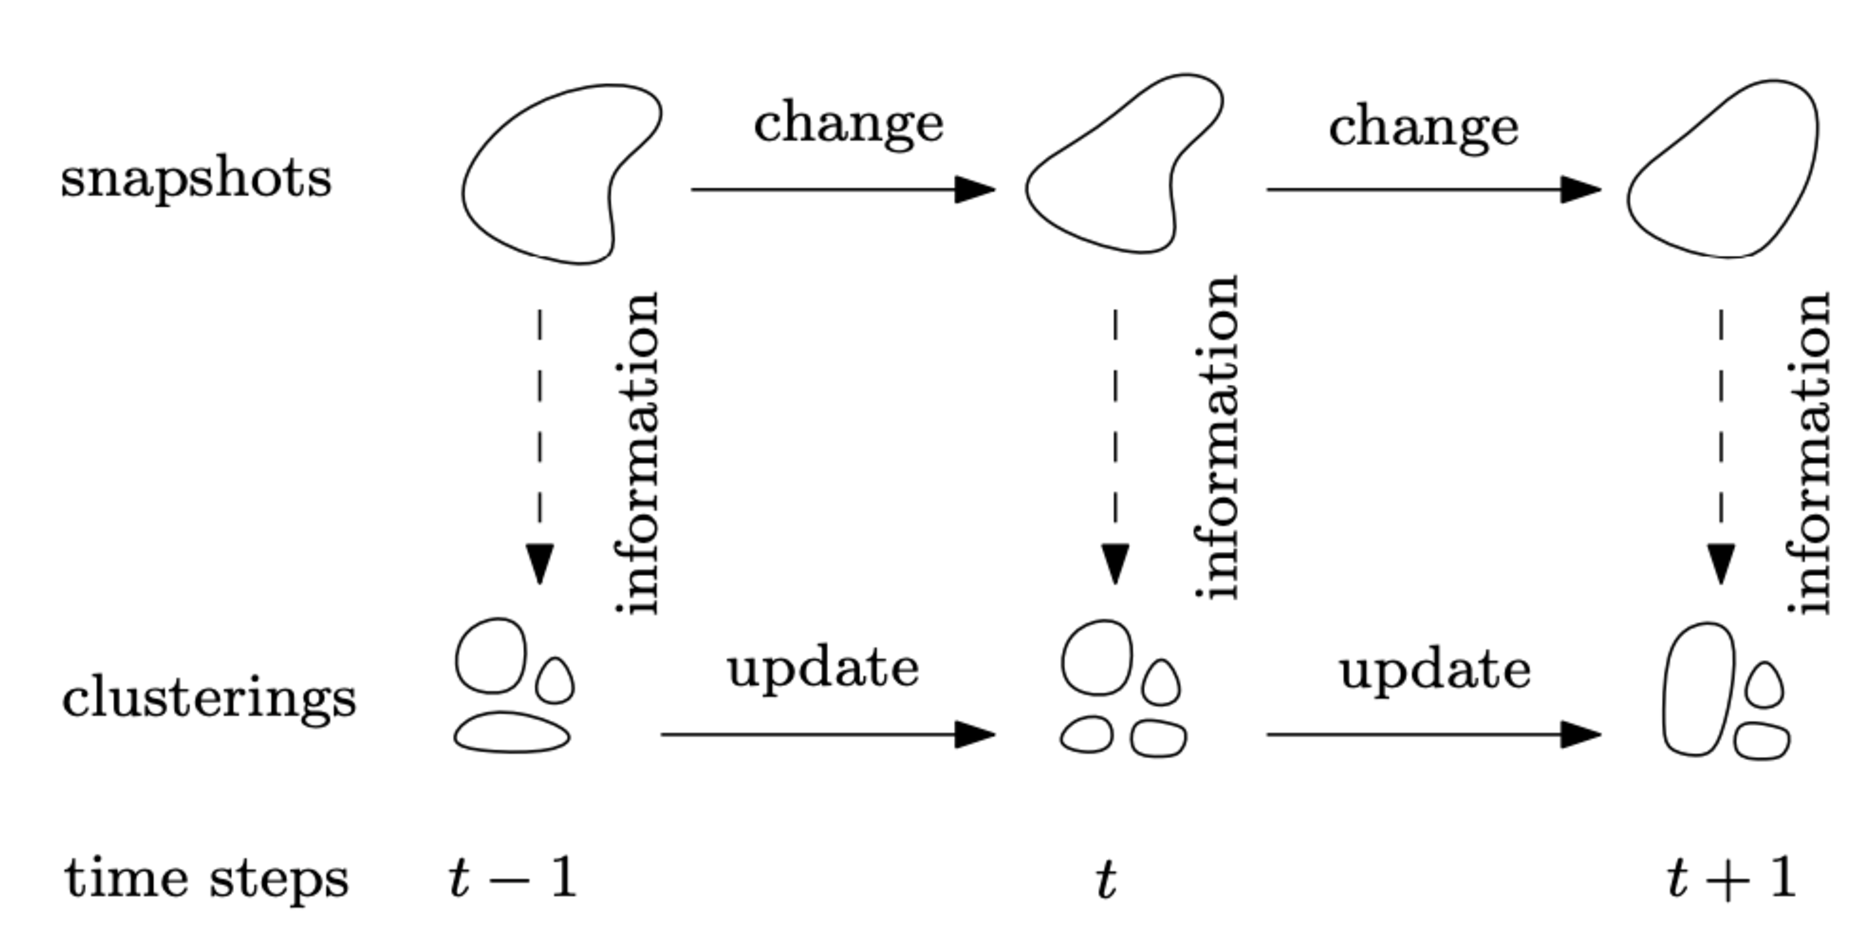
\includegraphics[width=0.9\columnwidth]{img/chapter2/dynamic.pdf} 
 	\caption{Dynamic community detection conventional steps. Figure is contributed from \cite{hartmann2016clustering}.}
 	\label{fig:c2_dynamic}
 \end{figure}  

\cite{chen2013detecting} is a classic study about dynamic community detection. It aims to learn a community matrix $C$ which best depicts the original graph adjacency matrix in a weighted form across all timestamps:
\begin{equation}
	\min_{Y}\sum_t \sum_{i,j}|A_{ij}-\frac{N_i N_j}{2|E|}||Y_{ij}-A_{ij}|
\end{equation}
where $Y=CC^T$.

DYNMOGA model \cite{folino2013evolutionary} is a genetic based approach to detect smooth communities with multi-object optimization. It considers the accuracy of the generated communities in the temporal graph at each timestamp. Meanwhile it also tries to minimize the transformation cost between two community partition results in consecutive timestamps. 

\cite{xu2014dynamic} combines two statistical models: a static model for individual graph snapshot in each timestamp and a temporal model to track the evolution of states. It proposes a prior \& posterior stochastic block model, in which the previously learned parameters in the last snapshot are used to optimize the current community memberships via  extended Kalman filter (EKF). Using similar approaches, SBTM model \cite{xu2015stochastic} leverages hidden Markov assumption in original SBM in which the presence/absence of an edge between two nodes will directly influence whether it will appear again in the next timestamp. 

NEIWalk model \cite{wang2013neiwalk} is a random walk method applied on dynamic content-based graphs by tracking the evolution of both graph structure and node/edge content.  In detail, the model transforms the original graph into a Node-Edge Interaction (NEI) graph which contains two types of nodes and three types of edges. In NEI graph, the two node types are the node and edge in the original content-based graph. And the three edge types are the calculated structural similarity, node content similarity and edge content similarity. The dynamics in the original content-based graph is reflected to the structure evolution in the NEI graph. To detect communities in each timestamp, a random walk based model is proposed to involve a transition probability matrix between each node/edge type and thereafter detect communities in the NMI graph. 

\cite{appel2018temporally} also detects dynamic communities in content-based graphs by incorporating graph structure, content and temporal analysis in a shared matrix factorization model. In each timestamp, it considers to learn three following matrices in a holistic way: a matrix $U_t$ at timestamp $t$ based on both structural and content information, a global  matrix $S$ based on structural information and another global matrix $W$ based on content information across all timestamps. The objective function uses these three matrices to best estimate the original adjacency matrix $A$ and given content matrix $C$:
\begin{equation}
\argmin \sum_{t}||A_t-U_tS^T||^2 + \beta\sum_{t}||C_t-U_tW^T||^2 + \lambda(||S||^2+||W||^2+\sum_t||U_t||^2)
\end{equation}
The first  term aims to estimate $A$, the second term aims to estimate $C_t$ at each timestamp $t$, and the third term is the regularization term  to avoid bias and overfitting.

\cite{wang2013dynamic} focuses on dynamic community detection in graph streams by defining a Local Weighted-Edge-based Pattern (LWEP), which is a subset of node densely connected in local regions. The whole approach is divided into online and offline steps. In the online step, for each node in timestamp $t$, a top-k neighbor node list (with largest edge weights) and a top-k candidate node list (with highest burst activities) are extracted to preserve graph main structure. In the offline step, the LWEPs are created in each timestamp from online results. A straightforward two-step approach first cleans the generated LWEPs and then uses a breadth first search (BFS) method to figure out dynamic community structures.  

\cite{kim2013nonparametric} proposes a nonparametric multi-group membership model for dynamic graphs. Within its model, a community can be tracked as either active or inactive, which is assumed to follows Poisson distribution. In timestamp $t$, the dynamic joining or leaving of a node towards a community is estimated by a Markov chain process considering its previous status in the community. The estimated parameters follow Beta distribution. The community structure can be used to estimate the probability of edge affinities in the original graph. Finally a MCMC method is used to optimize all the to-be-learned parameters under all assumed distributions.

\cite{ghasemian2016detectability} is a theoretical paper which argues a threshold generated from community strength and dynamic change rate. It claims that there would be no effective methods if the dynamic graph has a score below the threshold. Further more, it mathematically proves belief propagation model and spectral clustering are able to detect reliable communities if the graph structure is above the threshold.  

\cite{yang2018poisson} is another statistical work which assumes evolved node-community memberships following Gamma distribution. The communities also follows a Gamma distribution. The edges between nodes follow Bernoulli distribution and their weights follow Poisson distribution. The whole process optimizes all aforementioned distributions through a MCMC process. Similarly,  \cite{peixoto2017modelling} uses Bayesian Markov Chain to generate sequential edges appeared in the graph without specified time windows. 

\cite{delvenne2010stability} introduces a new metric, stability, to assess community partitions. The stability of a community partition is defined as:
\begin{equation}
	r(t,C) = \min_{0 \leq s \leq t} trace[C^T(\Pi M^t -\pi^T \pi)C]
\end{equation}
where $M$ is the node transition matrix, $\pi$ is the normalized degree vector over all nodes and$\Pi = diag(\pi)$ is the corresponding diagonal matrix. $C$ is the community  matrix. The partition with maximized stability may not be the best one in current timestamp. But its community structure should be with good coherence in a relative long time period.

In \cite{gauvin2014detecting}, the time-evolving graphs can be represented as a set of sequential adjacency matrices, which can be integrated as a three-way tensor $\mathcal{T}$. The conventional matrix factorization can be thereafter applied to the tensor by finding three low dimensional matrices $A,B,C$ to best estimate $\mathcal{T}$. $A$ and $B$ provides the graph community structure and $C$ represents the temporal activity of communities. It is a PARAFAC decomposition problem to solve.
\begin{equation} 
\min_{A,B,C} ||\mathcal{T} - A,B,C||^2_F
\end{equation}

\cite{tang2011identifying} focuses on dynamic multi-mode graphs, which is a particular type of heterogeneous graph where the node types and edge connections are constructed from different modes such as text and videos. It uses a matrix factorization approach to learn node community matrix in each timestamp by estimating the interaction between each pairwise modes. And a side effect from snapshot graph in the last timestamp are also considered in the learning process.

\subsection{Large Graph}

Large scale graphs are ubiquitous in various domains. Especially in recent years, with the increasing computation capability, more and more researches focus on how to deal with large graph community detection. A well-known survey paper \cite{harenberg2014community} introduces a number of methods focusing on both overlapping and disjoint community detection as well as many frequently used metrics and datasets for evaluation.

TopGC model\cite{macropol2010scalable} proposes a linear-time searching algorithm to detect the best community instead of the entire graph communities. It uses the idea derived from Locality Sensitive Hashing (LSH) to index nodes and find the communities with largest cluster scores (related to the community size and number of within-community edges). \cite{spielman2013local} is another local searching model which leverages random walks to detect the best community for each given node, and runs in approximately linear time. 

\cite{satuluri2011local} introduces a novel model to deal with large graphs by sparsifying graphs and removing unimportant edges to maintain the main graph structure. Once the graph size is reduced, the running time of most methods will be shortened as their complexity are always related to the graph size. To prune the graph in an efficient manner, a local sparsification algorithm is introduced to maintain the top ranked edges (edge score is calculated by the Jaccard Similarity of current node and the other endpoint node) per node. A further threshold is set up to ensure the pruned graph is still connected. 

\cite{wang2011detecting} formulates a novel problem, community kernel detection, which contains two tasks: find the most influential users and detect their community structure.
It proposes two separate algorithms, GREEDY and WEBA, both to solve the two tasks in a unified framework. In the GREEDY method, it firstly initializes a set of seed nodes as kernel communities. Then these communities expands by merging nodes with closest connections. In the WEBA method, the model learns a weight vector for each node to represent its belonging score to each community. The weight vectors are learned by maximizing the inner product of the vector of all pairwise connected nodes.

GEM model \cite{whang2012scalable} is proposed to cluster large-scale social networks. It consists of three steps: firstly it extracts the main skeleton from the original graph, and then detects the  skeleton graph communities via a k-means method, in the last step the calculated result is propagated back to refine the communities of entire graph. In detail, for graph extraction,  all nodes whose degree are above a threshold are selected and their edges are kept. Then a weighted k-means with refined seeding strategy is applied to cluster the filtered skeleton graph.  In the end, the remained nodes in the original graph are assigned to the generated communities through a breadth first search (BFS) approach.

\cite{li2013efficient} gives a novel definition of a community in which all nodes are closer to the current community centers than to the rest communities. After that, two new algorithms (Cores-Aware and Cores-Unaware algorithm) are proposed to detect communities in linear time. The Cores-Aware algorithm is leveraged under the condition that community cores are known. Then a breadth first search (BFS) approach is applied to calculate other node distances towards all cores and assign their communities. In the Cores-Unaware algorithm, their is no prior-known community cores. 

ESCG model \cite{liu2013large} repeatedly generates supernodes with coarser resolution to replace the original nodes in bipartite graph, which reduces the original graph size and accelerate the running speed. In detail, the model first randomly picks up a number of seed nodes as individual supernodes. Then a BFS approach is taken to allocate the rest nodes to the seed nodes based on their shortest paths. In the end, a standard spectral clustering method is leveraged on the reduced graph to detect communities. 

\cite{de2014mixing} proposes a mixed global and local method to bump up the efficiency via a defined k-path edge centrality as a substitution of the original edge betweeness centrality. Each edge importance score is calculated via random walks, which maps nodes to a latent space and calculates all pairwise distances for final community detection. The k-path edge centrality is defined as:
\begin{equation}
	L^k(e_{ij}) = \sum_{v \ V} Pr(e,v)
\end{equation}
It calculates the sum of probabilities that a k-step random walk passes edge $e_{ij}$ which is originally started as node $v$. And the distance of pairwise nodes can be thereafter calculated as:
\begin{equation}
	d_{ij} = 1 - \sqrt{\sum_{v \in V}\frac{(L^k(e_{vi})-L^k(e_{vj}) )^2}{d(v)}}
\end{equation}
The Louvain method is finally applied on the all pairwise node distances to calculate their communities.

\cite{kollios2013clustering} deals with large probabilistic graphs in which each edge is associated with a probability to appear or not appear. It proposes a simple model to generate a cluster graph $C$ which has the least edit distance with the original graph $G$. And the disjoint subgraphs in the cluster graph $C$ naturally form the communities.

SCD model \cite{prat2014high} is a scalable approach to detect communities by maximizing the Weighted  Community Clustering (WCC) metric. It also allows to run in parallel, which achieves a two-order magnitude acceleration in terms of running speed. WCC is defined based on the intuition that nodes should have a higher chance to form triangles with in-community nodes compared with the out-community nodes. Therefore, for a given node $v$, its WCC score in a community $c$ is calculated as:

\begin{equation}
WCC(v,c) = 
\begin{cases}
\frac{t(v,c)}{t(v,V)} \cdot \frac{vt(v,V)}{|c - v| + vt(x, V-c)} & \text{if t(v,V) $\neq$ 0}\\
0& \text{if t(v,V) = 0}
\end{cases}
\end{equation}
$t(v,c)$ and $t(v,V)$ refer to the number of triangles containing node $v$ in the community $c$ or the whole graph nodes. $vt(v,V)$ refers to the number of nodes that forms close triangles with current node $v$. The sum of all nodes' WCC scores across all communities is the final score to evaluate the fitness of current partition. The paper uses an iterative approach to learn the community partition with largest WCC score. \cite{tsourakakis2017scalable} also takes advantage of closed triangles in a spectral clustering approach.

\cite{li2015uncovering} aims to find overlapping communities in large-scale graphs. It defines a local spectra which uses a set of seed nodes (with known communities) as the dimensions to represent all other nodes through random walks. The local spectra representation hugely reduces the workload to decompose the adjacency matrix. And a refined k-means method helps to group nodes into overlapped communities. 

DFuzzy model \cite{bhatia2018dfuzzy} leverages deep learning techniques in four steps. First, it uses a PageRank method to initialize the potential community centers. Second,  PageRank based clustering encodes node hidden representations by maximizing graph Modularities. Communities are detected in the decoding process by minimizing the reconstruction error in the unified encode-decoder framework.

Some other studies are relevant to large-scale graphs from different perspectives. \cite{hallac2015network} is a theory paper which introduces network lasso to enhance the optimization process. \cite{jeub2015think} is an empirical paper aims to identify under what scenarios that small communities are better/equal/worse than large communities. \cite{peixoto2015model} offers a model selection strategy by considering graph minimum description length. 

\subsection{Attribute Graph}

\begin{figure}
	% \setlength{\belowcaptionskip}{-10pt}
	\center
	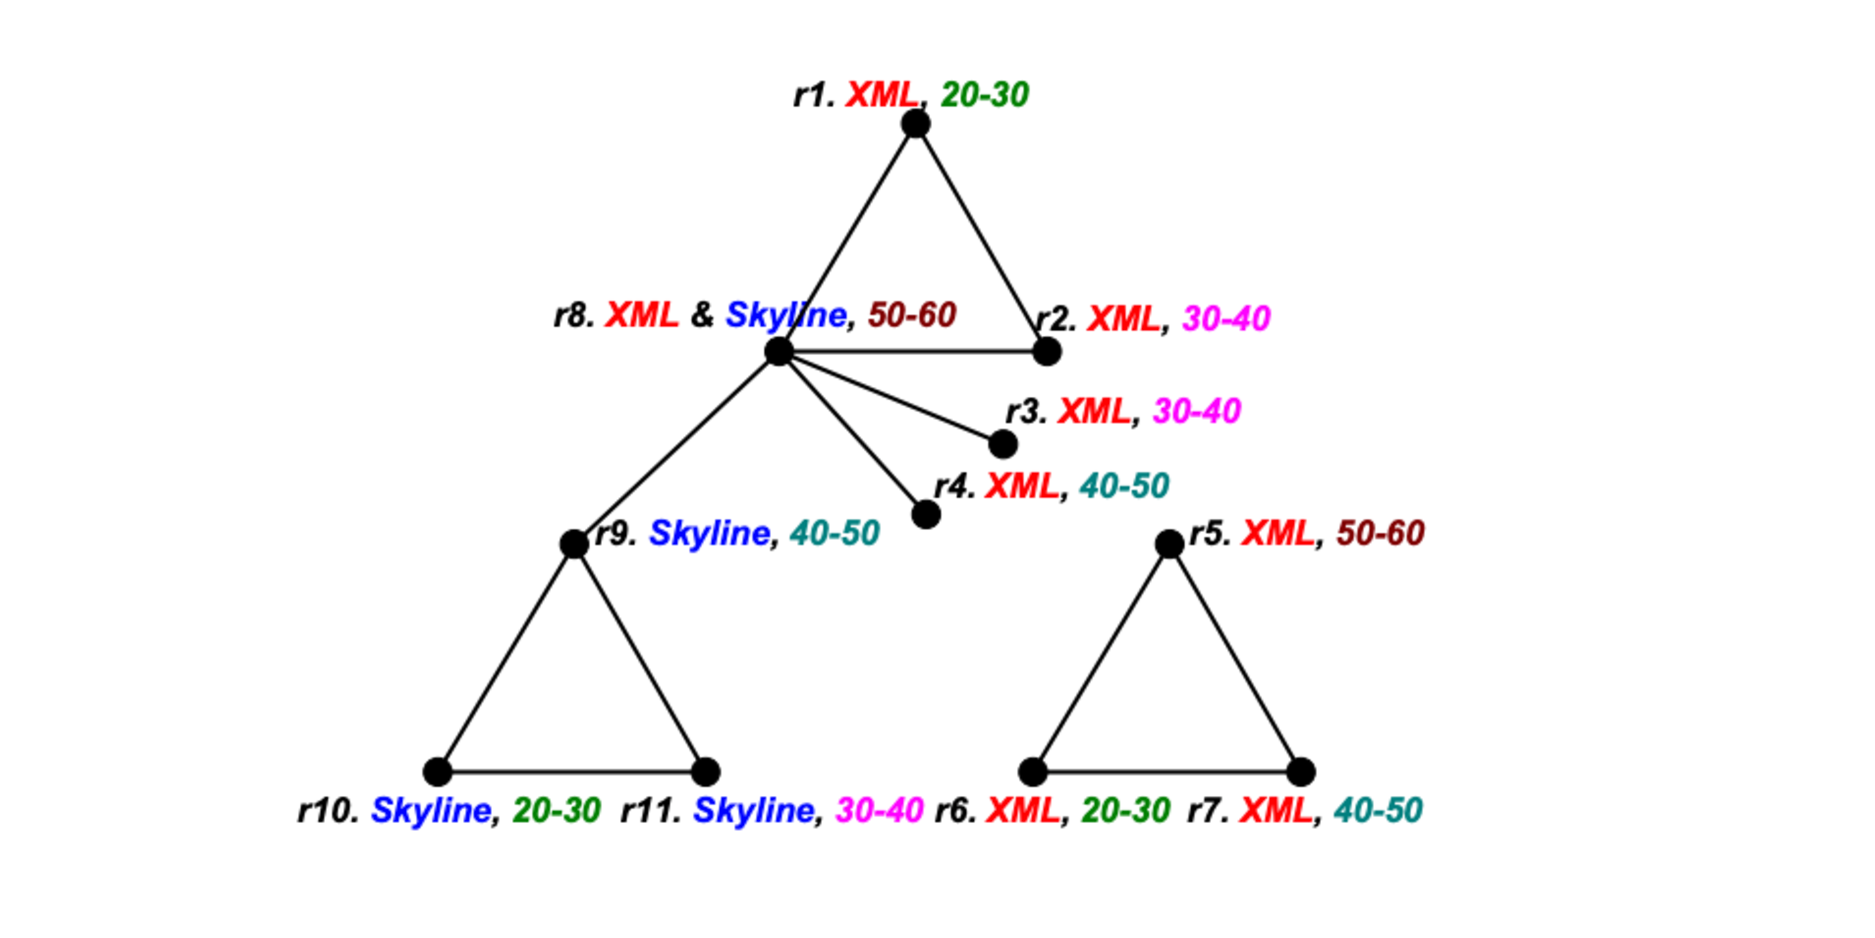
\includegraphics[width=\columnwidth]{img/chapter2/attribute.pdf} 
	\caption{A co-author graph with two attributes ``Topic'' and ``Age''. Figure is contributed from \cite{yang2013community}.}
	\label{fig:c2_attribute}
\end{figure}  


Intuitively, attribute graph is a type of graph in which nodes contains extra information. Figure \ref{fig:c2_attribute} shows a typical attribute co-author graph with ``Topic'' and ``Age'' attributes. An attribute graph $G(V,E)$ is associated with an attribute collection $\Lambda=\{ \lambda_1,...,\lambda_m\}$ containing $m$ different attributes.  Each node $v$ is associated with an attribute vector $[\lambda_1(v),...,\lambda_m(v)]$ where $\lambda_1(v)$ is the attribute value of node $v$ on attribute $\lambda_m$. A more complex attribute graph can involve attributes in edges as well with similar representations to node attributes.  Bayesian approaches and nonnegative matrix factorization approaches are the two main tracks of methods, and their related works are summarized in Table \ref{tab:c2_attribute}.

\begin{table}
	% \scriptsize
	\centering
	%   \vspace{-3em} 
	% \renewcommand{\tabcolsep}{2pt}
	\begin{tabular}{|p{5cm}|p{9cm}|} \hline
		\textbf{References} &  \textbf{Main Idea} \\ \hline
		\cite{xu2012model,han2015probabilistic,bojchevski2018bayesian,he2017joint} & Bayesian generative \& probabilistic model\\ \hline
		\cite{qi2012community,wang2016semantic,qin2018adaptive,}& Nonnegative matrix factorization\\ \hline
		\cite{zhang2019attributed,jin2019graph}& Graph convolutional network \\ \hline 
		\cite{zhou2010clustering,pool2014description,yang2013community,huang2015dense}& Others\\ \hline 
	\end{tabular}
	\caption{The main ideas of mainly introduced attribute graph community detection approaches.}
	\label{tab:c2_attribute}
	
\end{table} 


Inc-Cluster model \cite{zhou2010clustering}  uses random walk distance matrix instead of adjacency matrix to calculate node communities. The random walk distance matrix considers the random walk probability between each pair of nodes and their involved attributes. Thereafter, a Kmeans-like method is taken to initialize community centroids and run with the four following steps iteratively until convergence: first,  it assigns nodes to the community with the nearest centroid random walk distance; second, it updates each community centroid from the newly formed communities; third, it adjusts attribute weights with an efficient incremental method; fourth, it re-computes the random walk distance matrix and starts the next iteration. 

SCMAG model \cite{huang2015dense} aims to retrieve the dense communities from attribute graphs. It firstly leverages an entropy-based method to find dense subspaces. A random walk based method calculates the structural closeness and attribute similarity between communities together as a unified metric. A combining strategy is finally proposed based on the metric to merge subspaces together as communities. 

\cite{xu2012model} seamlessly captures both structural and attribute aspect information and develops a Bayesian probabilistic model to detect node communities. It leverages three matrices including adjacency matrix $X \sim Bernoulli(\cdot)$, attribute matrix $Y \sim Multinomial(\cdot)$ and node community label vector $Z \sim Multinomial(\cdot)$. The overall generative process firstly samples the community label for each node. Then given the community label and node itself, the model samples node attributes. In the end, given community labels for each pair of nodes, the model samples whether there is an edge between them. The overall idea is to reproduce the original graph by optimizing these three generation probabilities.

CRM model  \cite{han2015probabilistic} is also a probabilistic model to incorporate all user information from social networks. The overall approach aims to generate three types of user information including community (each edge belongs to a community), role (each node can have multiple roles) and action (edge node can take multiple actions such as transferring a message). The three generative process are interacted with each other and optimized through an EM approach. 

PAICAN  \cite{bojchevski2018bayesian} is a jointly model which learns partial node anomalies and communities via a statistical inference perspective. A node is a partial node anomaly when it is an outlier in at least one attribute. In the graph generative process, an edge is generated from different distribution assumption under three case of endpoint node information: both nodes are good,  one endpoint node is good, and both nodes are anomaly. \cite{he2017joint}  is another model involving node semantics. Similarly, the overall process is a joint community $\rightarrow$ edge generation and topic $\rightarrow$ attribute generation model.
 
\cite{pool2014description} aims to detect top $k$ communities which can both group cohesively connected nodes together and concisely describe their attributes. It defines two types of errors to assess community partition fitness. The first type error is missing edges between nodes in the same community. The second type error is the edges existing between communities. The model calculate the scores of community given these two criteria. The idea of this paper is to generate concise queries from node attributes and selects top $k$ best fit communities for these queries. 

CESNA model \cite{yang2013community} detects overlapping communities by considering both edge structure and node attributes. It is a scalable algorithm with linear running time. The intuition behind CESNA model is that node community memberships should be able to indicate node attributes. The probability that a node $u$ contains attribute $k$ is described as:
\begin{equation}
	P_{uk} = \frac{1}{1+exp(\sum_c W_{kc}\cdot F_{uc})}
\end{equation}
where $F_{uc}$ is the affiliation score that node $u$ belongs to community $c$. Weight $W_{kc}$ is the weight factor for attribute $k$ towards community $c$.

\cite{qi2012community} shows how edge content can be used to improve the effectiveness of community detection. The overall model is derived from matrix factorization. It considers to minimize both structural object and edge content object in a unified function $\mathcal{O}(E)$:

\begin{equation}
\mathcal{O}(E) = ||E^TE\Delta - \Gamma||^2_F - \lambda tr(E^TLE)
\end{equation}

The first part is the structural object to minimize, where $\Gamma$ is a $|E|\cdot|V|$  matrix to encode edge and node underlying structure. $\Gamma_{ij} = 1$ if $v_j$ is the start-or end-point of $e_i$. Otherwise $\Gamma_{ij} = 0$. $E$ is a low dimensional matrix representation for all edges. $\Delta$ is a  $|E|\cdot|V|$  matrix whose entry $\Delta_{ij} = \frac{1}{d(vj)}$ if $v_j$ is the start-or end-point of $e_i$. The second part is the edge content object. $tr(\cdot)$ denotes the trace of relevant matrix. $\lambda$ is a weighting factor. $L$ is the normalized Laplacian matrix storing all pairwise edge content similarities. In the end, edge vectors are learned  and used for community detection.

\cite{wang2016semantic} aims to learn a community membership matrix $U$ and community attribute matrix $C$ through a nonnegative matrix factorization framework. The objective function in this model is defined as:
\begin{equation}
	\argmin_{C \geq 0, U \geq 0}||U-SC||^2_F + \alpha\sum_{j=1}^{k}||C(:,j)||^2_F + \beta ||A-UU^T||^2_F
\end{equation}
where $U_{ij}$ is the propensity of node $i$ belongs to community $j$. $C_{qr}$ is the propensity of that attribute $q$ belongs to community $r$. $S$ is the given node attribute matrix. The first term aims to estimate node community membership matrix from node attributes. The second term is an add-on bias. The third term is to use community membership matrix to estimate the original adjacency matrix $A$.

\cite{qin2018adaptive} incorporates node content into a nonnegative matrix factorization approachc and use a weight matrix $C$ to control the impact of the attribute information for community detection. The objective function it aims to optimize is as:
\begin{equation}
\argmin_{X \geq 0,Y \geq 0} \alpha ||A-XX^T||^2_F + ||X-CY||^2_F
\end{equation}
where $A$ is the adjacency matrix, $X$ is the community membership matrix, $Y$ is the community attribute matrix to describe how much likely the community can be described by each attribute. $C$ is the node attribute matrix. Both $X$ and $Y$ are the matrices to be learned. 

\cite{zhang2019attributed,jin2019graph} are both deep-learning based method to involve node attribute into graph convolution process and trained in an end-to-end manner.

\subsection{Summary}
In this section, I introduce five different types of graphs and a bunch of related research works. Some of the graph types are commonly seen in real-world scenarios such as sparse and large graphs. Effective and efficient models on such graphs can produce huge practical value to reduce online latency and required machine memories. Researches in attribute graph is becoming more popular because it can involve extra information to support graph partition. The extra information is always with meaningful semantics, clear format and easy to be obtained.  Besides the type of graphs introduced in this section, there are also other types of works, such as signed graph and hypergraph, which are all interesting topics and deserves more future exploration.  